\newpage
\section{Information}
    Vielen dank an David Reiser, der mir sein Makefile zur Verfügung gestellt hat. 
    \\
    Weiterhin kann das komplette Projekt in folgender GITHUB Repository nachvollzogen werden: 
    \href{https://github.com/FabioPlunser/DIC-Lezuo/tree/master/2.Semester-serial_crypto/DIC-serial-crypto-Programm}{https://github.com/FabioPlunser/DIC-Lezuo/}

\section{Aufgabenstellung}
    Die Aufgabe ist es, im echtzeit Betriebssystem Zephyr einen Krypto Prozessor zu programmieren, der einen Verschlüsselten Text erhält und 
    mit AES-128 cbc entschlüsselt.
    Der Prozessor wird mit dem \textbf{nativ\_posix-Board} programmiert. Dieses kann in eine normal ausführbare Datei 
    kompiliert werden, die man auf einem Linux System ausführen kann. Somit wird ein Mikronroller Board emuliert.  
    

\subsection{Aufgaben und Eigenschaften des Krypto Prozessors}
    Der Krypto Prozessor soll in 4 Threads, \textbf{main, uart-in, uart-out, processing} aufgeteilt werden. Weiterhin soll die vorgegebene Statemachine und UART Protokoll implementiert werden. 
    Die Statemachine gibt vor in wann das Programm was machen soll. 
    \begin{figure}[!htb]
        \centering
        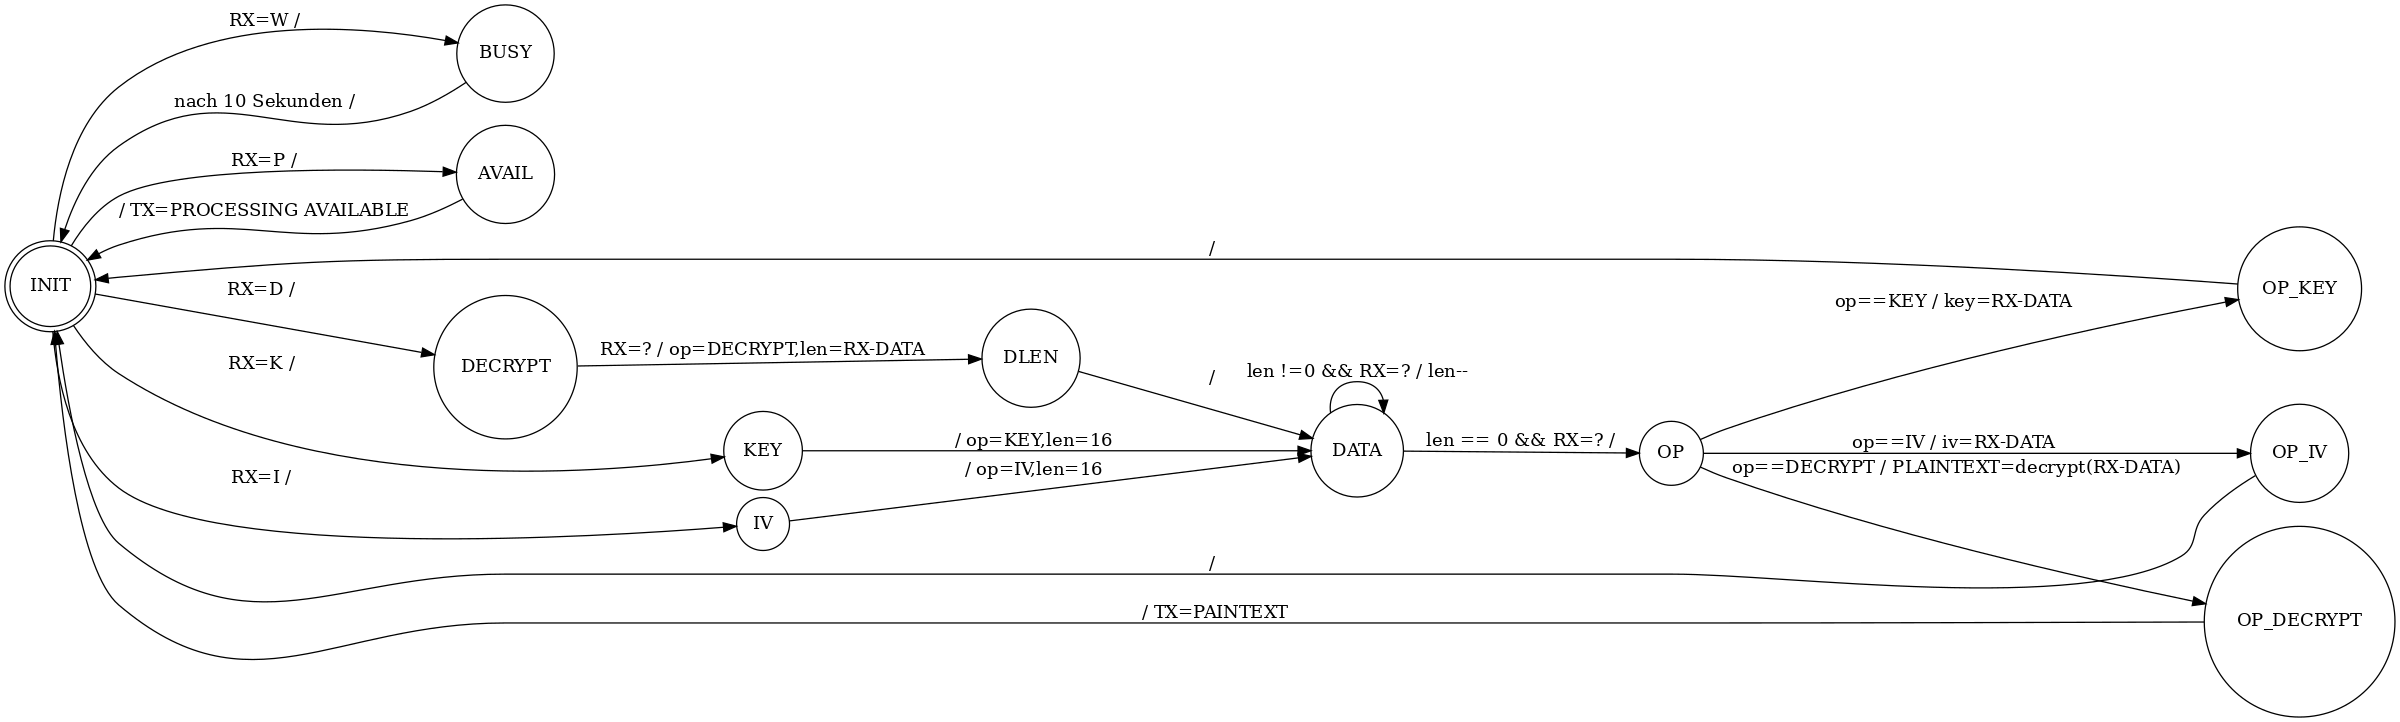
\includegraphics[width=\linewidth]{Statemachine.png}
        \caption{Statemachine}
        \label{caption:Statemachine}
    \end{figure}
    \\
    Weiterhin wurde ein UART Protokoll vorgegeben: 
    \begin{itemize}
        \setlength\itemsep{0em}
        \item alive: Wenn ein '.' empfangen wird, soll sofort ein '.' zurückgeschickt werden. 
        \item avail: Wenn ein 'P' empfangen wird, soll vom processing-thread \anfuehrung{PROCESSING AVAI} zurückgeschickt werden. 
        \item key: Wenn ein 'K' empfangen wird, folgen 16 Byte Des AES-128 Schlüssel, dieser empfangene Schlüssel wird in den Kryptoprozessor geladen.  
        \item iv: Wenn ein 'I' empfangen wird, folgen 16 Byte des AES-128 IV, , dieser empfangene IV wird in den Kryptoprozessor geladen.
        \item Decrypt: Wenn ein 'D' empfangen wird, gefolgt von der Länge des Ciphertextes, gefolgt vom Ciphtertext, wird dieser Ciphertext mit dem 
        entsprechenden Key und IV mit AES128-CBC entschlüsselt und als Plaintext an der UART ausgegeben. 
        Wenn der Ciphtertext nicht durch 16 Teilbar ist, soll eine Fehlermeldung \anfuehrung{XERROR} zurückgesendet werden. 
    \end{itemize}
    \noindent Das Programm soll alle Tests der vorgegebenen test.py Datei erfolgreich absolvieren. 
    Die Tests, testen ob die Statemchine korrekt implementiert wurde und besteht aus folgende Test: 
    \begin{itemize}
        \setlength\itemsep{0em}
        \item Test0: Testung der UART Verbindung, indem ein '.' Punkt an den Prozessor geschickt wird. 
        \item Test1: Testung der availibility, indem ein 'P' an den Prozessor geschickt wird. 
        \item Test2: Testung ob der Processor korrekt blockiert 
        \item Test3: Testung ob ein Error vom Prozessor zurückgeschickt wird, wenn ein absichtlich nicht funktionierender Ciphertext an den Prozessor geschickt wird, da dieser nicht durch 16 Teilbar ist. 
        \item Test4: Testung ob die standard Konfiguration der Entschlüsselt korrekt ist. 
        \item Test5: Testung ob ein anderer Key und IV von dem Prozessor übernommen wird. 
    \end{itemize}
    
